\documentclass{article}
\usepackage[utf8]{inputenc}
\usepackage{amsmath}
\usepackage{graphicx}
\usepackage{float}
\usepackage{multibibliography}
\begin{document}
\section*{CV Project \#2}
Name: Qiang Fu
\\Date: November 4th 2019
\subsection*{Introduction}
\par
In this project, we are asked to calculate the fundamental matrix given all the camera information as well as calculate it using 8-points method. The fundamental matrix is a 1 to n projection between image points on the two images. And for the second part we are asked to rectify the two cameras. After the rectification, the image points on the two images corresponding to the same 3D point will locate on the same image column of the rectified images. For the third part, we need to reconstruct 3D facial points from two images and all the camera information is known.
\subsection*{Calculating fundamental matrix F}
\par
There are two methods to calculate fundamental matrix F. The fisrt method is calculating F by definition $W_l^{-T}S^TRW_r^{-1}$. Using the same method from project 1, we can calibrate the two cameras and we can get $W_l,W_r,R,t$. The second method is the 8-points method.
\par
From the epipolar constraint that $P_l,P_r$ and the baseline must be coplanar, we can derive 
\begin{equation}
(t\times P_l)RP_r = 0
\end{equation}
And it can be written as
\begin{equation}
P_l^TS^TRP_r = 0
\end{equation}
where 
\begin{equation}
S = \begin{bmatrix}
0&-t_z&t_y\\
t_z&0&-t_x\\
-t_y&t_x&0
\end{bmatrix}
\end{equation}
and 
\begin{equation}
P_l = \lambda_lW_l^{-1}U_l,
P_r = \lambda_rW_r^{-1}U_r
\end{equation}
Then Eq.2 can be written as
\begin{equation}
U_l^TW_l^{-T}S^TRW_r^{-1}U_r=0
\end{equation}
and $W_l^{-T}S^TRW_r^{-1}$ is call fundamental matrix $F$.
\par
From project 1 we know that the projection matrix $P$ can be reconstructed from known 3D,2D points, and we can also exclude outliars by RANSAC method. Then the intrinsic matrix $W$, rotation matrix $R$, translation vector $t$ can be reconstructed from $P$. After knowing the intrinsic and extrinsic matrix, we can calculate the fundamental matrix by definition
\begin{equation}
F = W_l^{-T}S^TRW_r^{-1}
\end{equation}
The result is following.\\
For the left camera
\begin{align*}
W_l &= \begin{bmatrix}
1632&0&1056\\0&1600&753.1\\0&0&1
\end{bmatrix},
R_l = \begin{bmatrix}
-0.5105&0.8598&0.0115\\
0.1345&0.0606&0.9891\\
0.8497&0.5065&-0.1466
\end{bmatrix}
\\
t_l &= \begin{bmatrix}
9.8585&-28.9584&122.3561
\end{bmatrix}^T
\end{align*}
For the right camera
\begin{align*}
W_r &= \begin{bmatrix}
1620&0&1015\\0&1602&726.9\\0&0&1
\end{bmatrix},
R_r = \begin{bmatrix}
-0.8567&0.5157&0.0132\\
0.1255&0.1839&0.9749\\
0.5003&0.8368&-0.2223
\end{bmatrix}
\\
t_r &= \begin{bmatrix}
20.2861&-17.0725&119.3243
\end{bmatrix}^T
\end{align*}
We can find that the intrinsic matrix for the two cameras are not the same. This is because the focal length $f$, sampling rate $s_x,s_y$, image origin $c,r$ and distortion parameters are not the same for the two cameras.
\par
In order to calculate $F$, we need to calculate relative rotation and translation between the two cameras. And in this report all the relative rotations and translations are the rotaton and translation of the right camera relative to the left camera, denote as $R_{lr}$ and $t_{lr}$.
\begin{equation}
P_{Cl} =R_lP_W+t_l,P_{Cr} =R_rP_W+t_r
\end{equation}
And due to the coordinates in world frame are the same for the left and right camera, we can derive
\begin{align}
P_{Cl}&=R_lR_r^{-1}P_{Cr}+t_l-R_lR_r^{-1}t_r\\
R_{lr}&=R_lR_r^{-1}\\
t_{lr}&=t_l-R_{lr}t_r
\end{align}
Then from Eq.6 we can calculate the fundamental matrix F
\begin{equation*}
F=
\begin{bmatrix}
-4.6381e-07&1.0462e-5&-0.0097\\
1.6865e-06&-2.4980e-06&-0.0417\\
-0.0026&0.0289&10.2901
\end{bmatrix}
\end{equation*}
\par
We can also use the 8-points method to sovle the fundamental matrix. The basic idea is that we can solve 
\begin{equation}U_l^TFU_r=0\end{equation}
linearly using at least 8 points from each image. Write fundamental matrix $F$ as $F=\begin{bmatrix}F_1&F_2&F_3\end{bmatrix}$, where $F_1,F_2,F_3$ are the fisrt, second and third columns of $F$. Then we can rewrite Eq.11 as follow
\begin{equation}
\begin{bmatrix}
U_{li}^TF_1&U_{li}^TF_2&U_{li}^TF_3
\end{bmatrix}U_{ri}=0
\end{equation}
And furtherly we can rewrite Eq.12 as
\begin{equation}
\begin{bmatrix}
U_{li}^Tc_{ri}&U_{li}^Tr_{ri}&U_{li}^T
\end{bmatrix}\begin{bmatrix}F_1\\F_2\\F_3\end{bmatrix}=0
\end{equation}
If we have $N$ points we can construct a system of linear equations
\begin{equation}
\begin{bmatrix}
U_{l1}^Tc_{r1}&U_{l1}^Tr_{r1}&U_{l1}^T\\
 &\vdots& \\
 U_{lN}^Tc_{rN}&U_{lN}^Tr_{rN}&U_{lN}^T
\end{bmatrix}\begin{bmatrix}F_1\\F_2\\F_3\end{bmatrix}=0
\end{equation}
And with at least 8 points we can solve $F$ up to a scale factor. And there is no constraint on the scale factor\cite{ref1}. However the findamental matrix we calculated denotes as $F_{cal}$ may not have the property of $F$ that the rank of $F$ is 2. Then we need to add the constrint by applying SVD to $F_{cal}$ and force the third singular value to be 0 and reform the fundamental matrix denote as $F^*$.\cite{ref2} And the redult is as follow
\begin{equation*}
F^*=\begin{bmatrix}
-1.1545e-08&5.9903e-07&-9.8898e-04\\
2.3489e-07&-1.0073e-07&-0.0027\\
-3.4872e-04&0.0018&1
\end{bmatrix}
\end{equation*}
The fundamental matrix we get here is very different from the one we get by definition. The first reason is that $F^*$ is up to a scale factor. the second reason is that $F_{cal}$ does not meet the property of a fundamental matrix so we apply SVD to it and force the third singular value to be 0. And during this process there are errors intriduced. In order to see how large the error is, we define the error in the following way
\begin{equation}
E = U_l^TFU_r
\end{equation}
And we can visualize it as Figure 1
\begin{figure}[H]
\centering
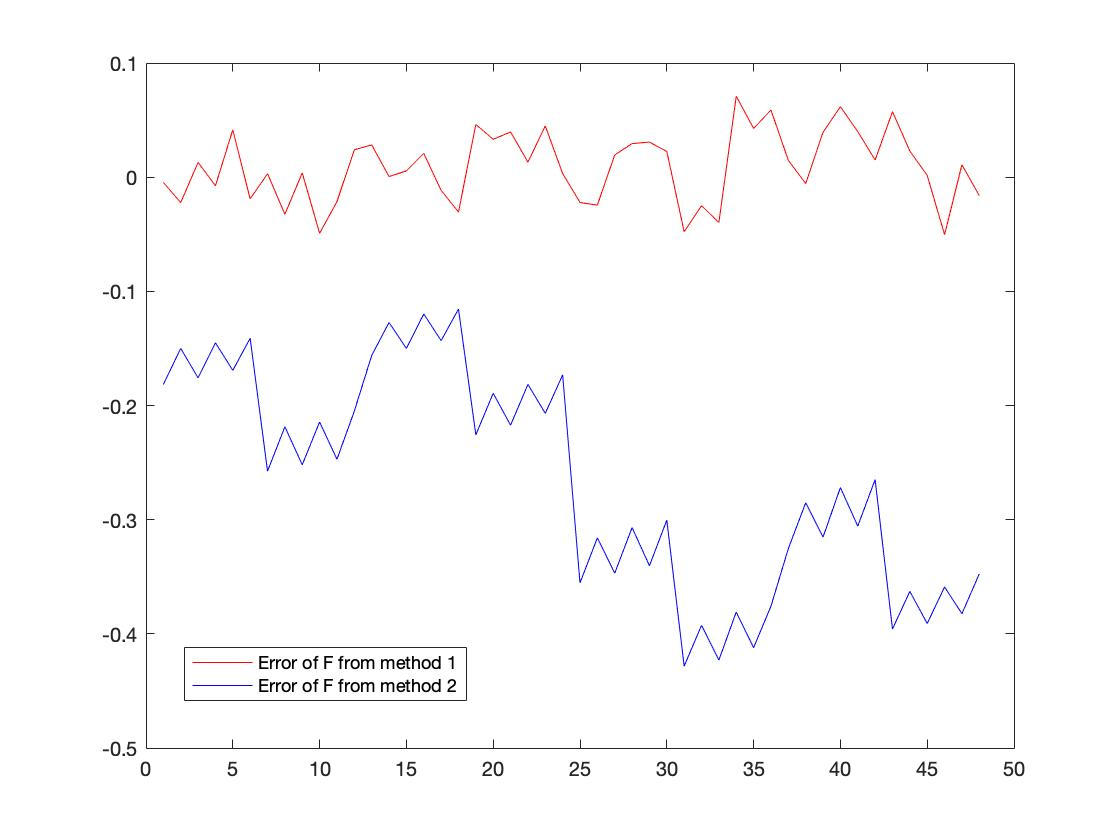
\includegraphics[scale=0.2]{Error.jpg}
\caption{Errors of fundamental matrix}
\label{fig:label}
\end{figure}
From Figure 1 we can see that the error of $F^*$ is much bigger than $F$.
\subsection*{Rectification}
\par
In practice, the image plane of two cameras are often chson to be coplanar and parallel to their base line. In this case the epipolar lines are parallel and conjugate epipolar lines are collinear. However it is hard to make the two image planes coplanar and parallel to the base line psysically since the origins of the two camera are inside and the image plane is a virtual plane. The method we use to make the two image plane coplanar is called rectify, and it is done digitally.\cite{ref1} 
\par
We can assume a rotation $R_{rec\_l}$ of the left camera, and after the rotation, the new X axis and the relative translation $t_{lr}$ are colinar. And for the right camera, we also apply a rotation $R_{rec\_r}$ on it, and the new X axis of the right camera is colinar with $t_{lr}$. And we can write the following equation
\begin{equation}
\begin{bmatrix}1\\0\\0\end{bmatrix}=R_{rec\_l}\frac{t_{lr}}{\left\|t_{lr}\right\|_2}
\end{equation}
which means
\begin{equation}
R_1 = \frac{t_{lr}^T}{\left\|t_{lr}\right\|_2}
\end{equation}
where $R_1$ is the first column of $R_{rec\_l}$, then we can construct $R_{rec\_l}$ that meets the properties of othorgonal matrix.
\begin{equation}
R_{rec\_l}=\begin{bmatrix}
t_x^*&t_y^*&t_z^*\\
t_y^*/\lambda&-t_x^*/\lambda&0\\
 &R_1\times R_2& 
\end{bmatrix}
\end{equation}
where $\begin{bmatrix}t_x^*&t_y^*&t_z^*\end{bmatrix}=\frac{t_{lr}^T}{\left\|t_{lr}\right\|_2}$, $\lambda = \sqrt{(t_x^*)^2+(t_y^*)^2}$ and $R_1,R_2$ are the first and second column of $R_{rec\_l}$. And for the right camera, since it has the same orientation with the left camera after rectifying, so the rectifying matrix for the right camera can be easily got as 
\begin{equation}
R_{rec\_r}=R_{rec\_l}R_{lr}
\end{equation}
And for the image points before and after rectifying, we have
\begin{align}
\lambda_l^*\begin{bmatrix}c_l^*\\r_l^*\\1\end{bmatrix}&=W_l\begin{bmatrix}X_{cl}^*\\Y_{cl}^*\\Z_{cl}^*\end{bmatrix}\\
\lambda_l\begin{bmatrix}c_l\\r_l\\1\end{bmatrix}&=W_l\begin{bmatrix}X_{cl}\\Y_{cl}\\Z_{cl}\end{bmatrix}\\
\begin{bmatrix}X_{cl}^*\\Y_{cl}^*\\Z_{cl}^*\end{bmatrix}&=R_{rec\_l}\begin{bmatrix}X_{cl}\\Y_{cl}\\Z_{cl}\end{bmatrix}
\end{align} 
Combine Eq.20, Eq.21 and Eq.22, we have
\begin{equation}
k_l\begin{bmatrix}c_l^*\\r_l^*\\1\end{bmatrix}=WR_{rec\_l}W_l^{-1}\begin{bmatrix}c_l\\r_l\\1\end{bmatrix}
\end{equation}
also we can derive the relationship for the right camera 
\begin{equation}
k_r\begin{bmatrix}c_r^*\\r_r^*\\1\end{bmatrix}=WR_{rec\_r}W_r^{-1}\begin{bmatrix}c_r\\r_r\\1\end{bmatrix}
\end{equation}
where $W=\frac{1}{2}(W_l+W_r)$, because we need to make sure the intrinsic parameters are the same for both camera after rectifying. Then with Eq.22 and Eq.23 we can map the points before and after rectifying. 
\par 
To generate the rectified image, we can use back forward mapping. The main idea of this method is that for each pixel on the rectified image, we can find the corresponding pixel on the original image using Eq.22 or Eq.23 and if the corresponding pixel on the original image is beyond the image then the rectified pixel is a black pixel. And from project 1 we know how to calculate the epipolar lines, then we can draw the images before and after the rectification and the facial points' corresponding epipolar lines.
\begin{figure}[H]
\centering
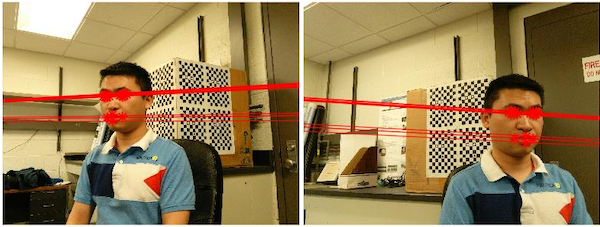
\includegraphics[scale=0.55]{1.png}
\caption{Left and right images before rectification}
\label{fig:label}
\centering
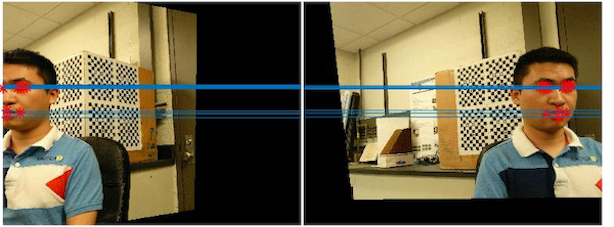
\includegraphics[scale=0.55]{3.png}
\caption{Left and right images after rectification}
\label{fig:label}
\end{figure}
And from the Figure 2 and Figure 3, we can see that the result is pretty good,the epipolar lines before rectification are not parallel and the corresponding points between the two original images are not at the same image column. And after the rectification the epipolar lines are parallel and the corresponding points between two images are at the same image column. And after rectification, the point matching will be much easier.
\subsection*{Reconstruction}
\par
The major task for this part is to calculate the 3D coordinates of the facial points given their 2D coordinates in two images. We can use full reconstruction method since all the camera parameters are known. For each point we have
\begin{equation}
\lambda_l\begin{bmatrix}c_l\\r_l\\1\end{bmatrix}=\begin{bmatrix}P_{l1}&P_{l14}\\P_{l2}&P_{l24}\\P_{l3}&P_{l34}\end{bmatrix}\begin{bmatrix}X\\Y\\Z\\1\end{bmatrix}
\end{equation}
And we can rewrite Eq.25 as 
\begin{align}
\lambda_lc_l=P_1\begin{bmatrix}X\\Y\\Z\end{bmatrix}+P_{14}\\
\lambda_lr_l=P_2\begin{bmatrix}X\\Y\\Z\end{bmatrix}+P_{24}\\
\lambda_l=P_3\begin{bmatrix}X\\Y\\Z\end{bmatrix}+P_{34}
\end{align}
Then substitute $\lambda_l$ in Eq.26 and Eq.27 with Eq.28, we have
\begin{equation}
\begin{bmatrix}
c_lP_{l3}-P_{l1}\\r_lP_{l3}-P_{l2}
\end{bmatrix}\begin{bmatrix}
X\\Y\\Z
\end{bmatrix}=\begin{bmatrix}
P_{l14}-c_lP_{l34}\\P_{l24}-r_lP_{l34}
\end{bmatrix}
\end{equation}
Also for the right image we have the similar equation, and combine all the equations we have 
\begin{equation}
\begin{bmatrix}
c_lP_{l3}-P_{l1}\\r_lP_{l3}-P_{l2}\\c_rP_{r3}-P_{r1}\\r_rP_{r3}-P_{r2}
\end{bmatrix}\begin{bmatrix}
X\\Y\\Z
\end{bmatrix}=\begin{bmatrix}
P_{l14}-c_lP_{l34}\\P_{l24}-r_lP_{l34}\\P_{r14}-c_rP_{r34}\\P_{r24}-r_rP_{r34}
\end{bmatrix}
\end{equation}
Then for each point we have 4 equations and 3 unknowns, we can use the least squares method to solve it. And the result is as follow.
\begin{figure}[H]
\centering
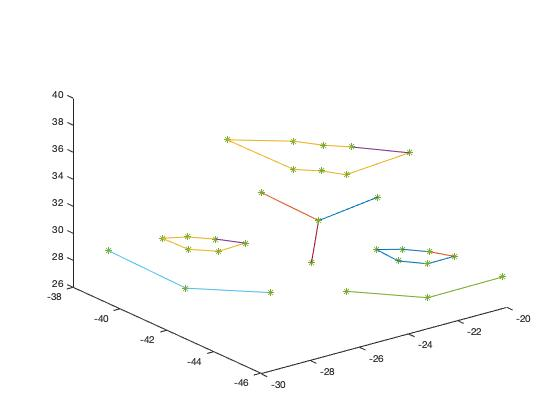
\includegraphics[scale=0.55]{face.jpg}
\caption{Reconstructed 3D facial points}
\label{fig:label}
\end{figure}
And the width of the left eye, right eye and mouth are 2.4620, 2.3595, 5.3791.
\subsection*{Summary and conclusion}
\par
In this project we did camera calibration, fundamental matrix reconstruction from 8-points method, camera rectification and 3D full reconstruction.
\par
In the first part, to reconstruct the fundamental matrix, we have two methods. If the points' 3D coordinates are known we can first calibrate the camera and then calculate the fundamental matrix by drfinition. And if the points' 3D coordinates are unknown, we can apply 8-points method to solve the fundamental matrix. However the result from 8-points method may not have the fundamental matrix's properties, so we need to apply the constraint additionally.
\par
In the second part, we applied camera rectification to the two images to make the image plane coplanar and parallel to the base line. And after calculating the rectification matrix, we can use the back forward mapping to generate the rectified image. However the back forward mapping is very time consuming.
\par
In the third part, we use the full reconstruction method to calculate the 3D facial points' coordinates.
\newpage
\begin{thebibliography}{}  
\bibitem{ref1}Qiang Ji. RPI ECSE 6650 Computer Vision, Lecture Notes: 3D Reconstruction. URL:https://www.ecse.rpi.edu/\~qji/CV/3dreconstruction2.pdf. Last visited on 2019/11/7.
\bibitem{ref2}Wikipedia contributors, "Eight-point algorithm"Wikipedia, the free encyclopedia, https://en.wikipedia.org/wiki/Eight-point_algorithm(accessed November 7,2019).
\end{thebibliography}
\end{document}